\documentclass[journal,12pt,twocolumn]{IEEEtran}
\usepackage{graphicx}
\graphicspath{{./figs/}}{}
\usepackage{amsmath,amssymb,amsfonts,amsthm}
\newcommand{\myvec}[1]{\ensuremath{\begin{pmatrix}#1\end{pmatrix}}}
\usepackage{listings}
\usepackage{watermark}
\usepackage{titlesec}
\let\vec\mathbf

\titlespacing{\subsection}{0pt}{\parskip}{-3pt}
\titlespacing{\subsubsection}{0pt}{\parskip}{-\parskip}
\titlespacing{\paragraph}{0pt}{\parskip}{\parskip}
\newcommand{\figuremacro}[5]{
    
}
\lstset{
frame=single, 
breaklines=true,
columns=fullflexible
}
\thiswatermark{\centering \put(0,-105.0){
\includegraphics[scale=0.5]{iith.png}} }

\sloppy
\title{\mytitle}
\title{
Matrix Assignment - Circle
}
\author{Nikhil Nair}
\begin{document}
\maketitle
\tableofcontents
\bigskip


\section{\textbf{Problem}}
If  a circle passes through the point (a,b) and cuts the circle $x^2+y^2=4$ orthogonally, then the locus of its centre is .\\


\section{\textbf{Solution}}
The equation of a circle is given as,   \\

${\vec{x^{\top}V_1 x} + 2\vec{u_1^{\top}x}} + f_1=0$
\\
\\
The circle given in the question can be written in the above form as follows
\\

$\myvec{x & y}\myvec{1&0\\ 0&1}\myvec{x\\y} + 2\myvec{0&0}\myvec{x\\y} + f_1 = 0$\\
\\
where,
\\

$\vec{V_1}=\myvec{1&0\\ 0&1} ; \vec{u_1^{\top}}=\myvec{0&0} ; f_1=-4$
\\
\\

Given that the two circles are orthogonal, therefore
\\
\begin{center}
$r_1^2 + r_2^2 = {\lVert \vec{u_1} - \vec{u_2} \rVert}^2$
\end{center}

\begin{equation}
r_1^2 + r_2^2 = {\lVert \vec{u_1} \rVert}^2 -{\lVert \vec{u_2} \rVert}^2 -2 \vec{ u_1}^{\top}\vec{u_2} \label{eq-1}
\end{equation}

\vspace*{1cm}
$r_1=2$ and $r_2$ are the radius of the given circles 
\\
\\
Now, we know
\begin{equation}
r_2=\lVert{ \vec{u_2} - \vec{L}}\rVert
\end{equation}             \label{eq-2}
\\
where L is a point (a,b) on the circle 2
\\
\\
$\vec{u_2}$ i.e centre of 2nd circle is taken as $\myvec{g&t}$

\begin{equation}
r_2^2=\lVert{ \vec{u_2}}\rVert^2+\lVert{ \vec{L}}\rVert^2-2\vec{u_2}^{\top}\vec{ L}                  \label{eq-3}  
\end{equation}            
\\
Solving $\ref{eq-1}$ and $\ref{eq-3}$ we get,\\

\begin{center}
$ r_1^2+\lVert{\vec{L}}\rVert^2-2\vec{u_2}^{\top}\vec{L}= 0$
\end{center}
\vspace{0.4cm}

$r_1^2+\vec{L}^{\top}\vec{L}-2\vec{u_2}^{\top}\vec{L}=0$
\\
\\

$r_1^2+\myvec{a&b}\myvec{a\\b}-2\myvec{g\\t}\myvec{a&b}=0$
\\
\\

$r_1^2+a^2+b^2-2ga-2tb=0$
\\
\\

Therefore the locus of the center of circle2 is
\\
\begin{center}
$2ga+2tb-(a^2+b^2+4)=0$
\end{center}

\vspace*{3.5cm}

\section{\textbf{Figure}}
\vspace*{1cm}
\begin{figure}[h]
    \centering
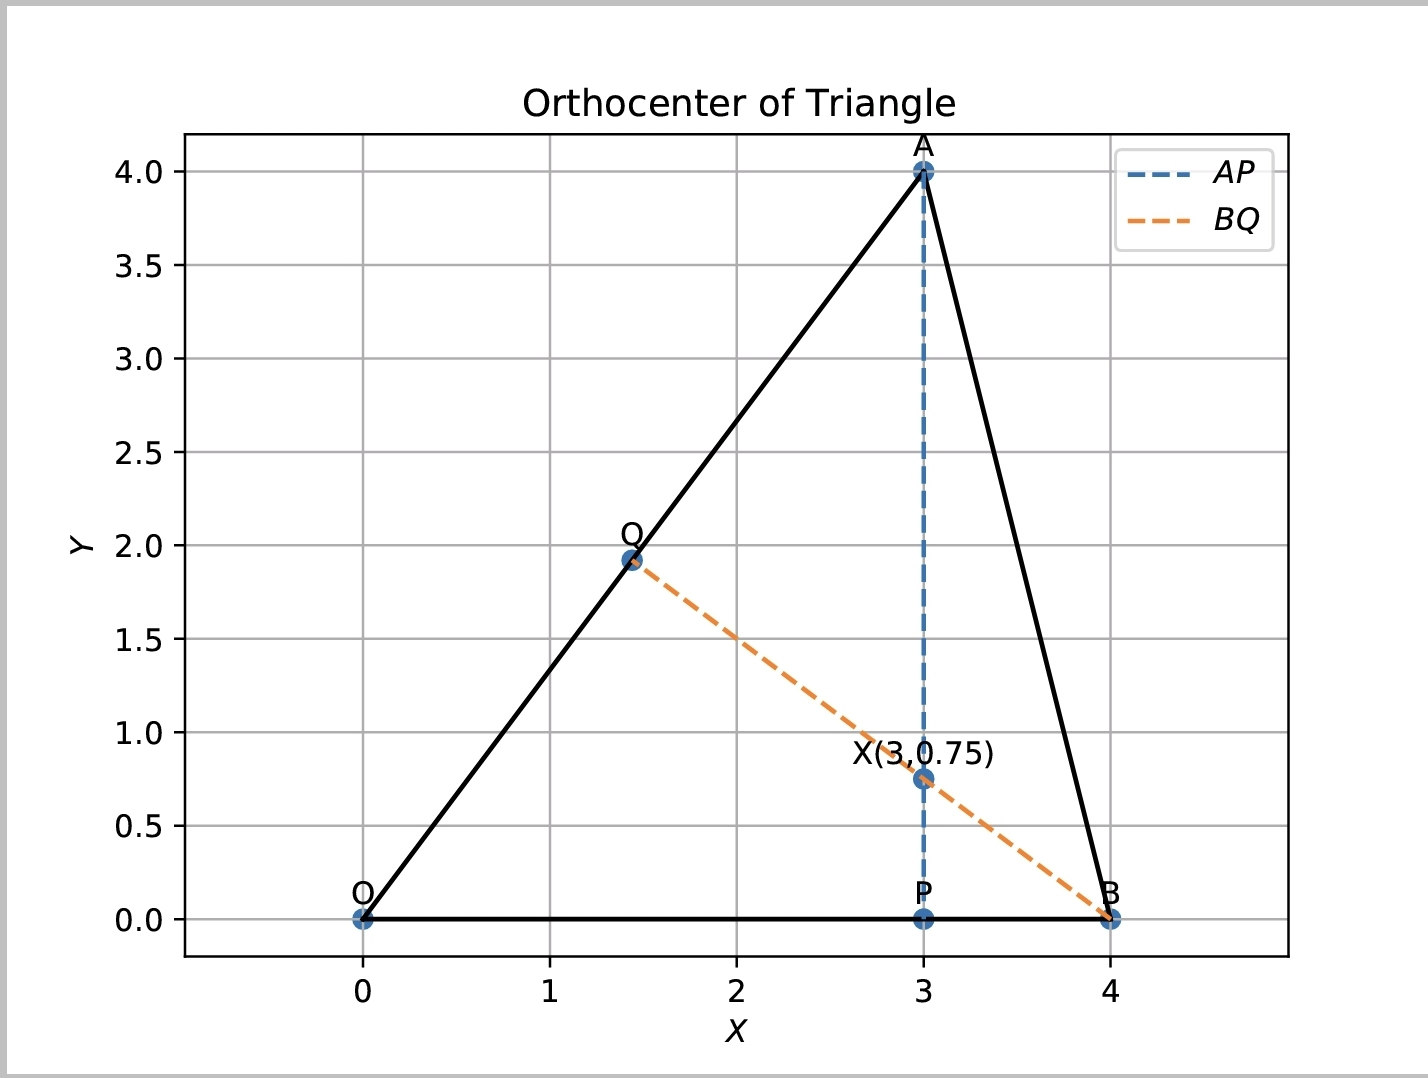
\includegraphics[width=\columnwidth]{fig.jpg}
    \label{fig:my_label}
\end{figure}


\section{\textbf{Code Link}}

\begin{lstlisting}
https://github.com/nikhilnair90/FWC-2/blob/main/Matrix/Circle/circle.py
\end{lstlisting}
Execute the code by using the command\\
\textbf{python3 circle.py}



\end{document}
